\documentclass[11pt,a4paper]{article}
\title{HDB++}
\author{Lorenzo Pivetta}
\date{\today}

\usepackage{svn-multi}
\svnRegisterAuthor{pivetta}{Lorenzo Pivetta}
\svnid{$Id$}

\usepackage{amsmath}
\usepackage{amsthm}
\usepackage{amsfonts}
\usepackage{amssymb}
\usepackage{color}
% \usepackage[dvips]{graphicx}
\usepackage[pdftex]{graphicx}
\usepackage{fancyhdr}
\usepackage{float}
\usepackage{hangcaption}
\usepackage{latexsym}
\usepackage{fancyvrb}
\usepackage{listings}
\lstset{
	basicstyle=\scriptsize\ttfamily,
	columns=flexible,
	breaklines=true
}
\usepackage{pdfpages}
% \usepackage{draftwatermark}
% \SetWatermarkText{Draft}
%% \SetWatermarkFontSize{4cm}
% \SetWatermarkScale{6}

\topmargin			0mm
\textheight 		230mm
\textwidth			145mm
\evensidemargin 0mm
\oddsidemargin  10mm
\headheight 		0mm
% \footheight 		10mm

\pagestyle{fancyplain}

\def \rev{Rev. 1.7}

\def \hdb{HDB++}
\def \es{Event Subscriber}
\def \esrel{ES}
\def \cm{Configuration Manager}
\def \cmrel{CM}
\def \de{Data Extraction}
\def \derel{DE}
\def \delrel{DEL}
\def \dbrel{DB}

\def \tango{TANGO}

\newcommand{\unit}[1]{\thinspace{#1}}
\newcommand\userinput[1]{\textbf{#1}}

\renewcommand{\familydefault}{\sfdefault}
\renewcommand{\sectionmark}[1]{\markright{\thesection \ \ #1}}
\lhead[\fancyplain{}{\rm\thepage}]{\fancyplain{}{\it\rightmark}}
\rhead[\fancyplain{}{\it\leftmark}]{\fancyplain{}{\rm\thepage}}

\lfoot[\fancyplain{}{\footnotesize}]{\fancyplain{}{\textit{
	\hdb{} \tango{} Device Server Design And Implementation
}}}
\rfoot[\fancyplain{}{\footnotesize}]{\fancyplain{}{\textit{
	Rev. \svnrev
}}}
\cfoot{}


\begin{document}

% \maketitle

\thispagestyle{empty}
\begin{center}
	\hspace{1.5cm}
	\emph{\tango{} Device Server Design Guidelines}
	\vspace{2cm}
	\newline
	\begin{LARGE}
		\textbf{\hdb} \\
	\end{LARGE}
	\vspace{1cm}
	\textbf{Design and implementation} \\
	\vspace{15cm}
	Changed by: \svnFullAuthor{\svnauthor} \\
	Date: \svndate \\
	Revision: \svnrev \\
	% Document URL: \svnmainurl \\
\end{center}

\newpage

\begin{Large}
	\textbf{Summary}
\end{Large}
\newline
The \hdb{} is a novel \tango{} device server for Historical Data Base
(HDB) archiving. It's written in C++ and is fully event-driven.
\vspace{2cm}

\begin{Large}
	\textbf{Keywords}
\end{Large}
\newline
\tango{} Device Server, Historical Data Base, HDB, Archiving, C++
\vspace{2cm}
	
\begin{Large}
	\textbf{Notes}
\end{Large}
\newline
No notes so far.
\vspace{2cm}

\begin{Large}
	\textbf{Contributions}
\end{Large}
\newline
R. Bourtembourg, J.M. Chaize, A.Gotz, J.Meyer, F.Poncet, E.Taurel, P.Verdier - ESRF
\newline
M.Lonza, C.Scafuri, G.Strangolino, L.Zambon - ELETTRA
\vspace{2cm}

\begin{Large}
	\textbf{Revisions}
\end{Large}
% \newline
\begin{table}[!htb]
	% \center
	\begin{tabular}{|c|c|c|l|}
		\hline
		\bf{Date} & \bf{Rev.} & \bf{Author} & \\
		\hline
		2012-12-04 & 1.0 & L.Pivetta & First release \\
		2013-01-29 & 1.1 & L.Pivetta & Merged suggestions from ESRF \\
		2013-01-31 & 1.2 & L.Pivetta & Cleanup \\
		2013-05-10 & 1.3 & L.Pivetta & Revision after HDB++ meeting on 14.03.2013 \\
		2014-01-30 & 1.4 & L.Pivetta & \cm{} details + Extraction library \\
		2014-03-07 & 1.5 & L.Pivetta & Database interface \\
		2014-05-05 & 1.6 & L.Pivetta & Cleanup, full ES and CM doc \\
		2014-07-28 & 1.7 & L.Pivetta & Revision after HDB++ meeting on 25.06.2014 \\
		2014-09-23 & 26520 & L.Pivetta & Moved to SVN \\
	\hline
	\end{tabular}
	\label{revisions}
\end{table}

\newpage{\clearpage}

\tableofcontents

\newpage{\clearpage}

% \listoffigures
\listoftables

\newpage{\clearpage}

\section{Historical Database}
The \tango{} Historical Database is a tool that allows to store the values
of \tango{} attributes into a database. The \tango{} core implements an
event-based interface to allow \tango{} device servers to publish the data
to be archived. The \textbf{archive} event can be triggered by two mechanisms:
\begin{itemize}
	\item delta\_change: the attribute value changed \emph{significantly}
	\item periodic: at a fixed periodic interval
\end{itemize}
The configuration parameters of each attribute, i.e. polling period, 
delta change thresholds, archiving period, are defined as properties
in the \tango{} database. In addition the archive event can be manually
pushed from the device server code.

For additional information concerning the \tango{} event subsystem
please refer to \emph{The \tango{} Control System Manual} Version 8.1.


\newpage{\clearpage}

\section{\hdb{} \tango{} Device Server}
The \hdb{} architecture is composed by several \tango{} device servers.
More in detail, at least one, but actually many, \es{} \tango{} device
server jointly with one \cm{} \tango{} device server and one or
more \de{} \tango{} device servers for each \tango{} domain are foreseen.

\subsection{Deployment best practices}
To take full advantage of the high performance and scaling capability
of the \hdb{} \tango{} device server some constraints have to be
taken into account.
Though a single instance of the \hdb{} device server is capable of
handling thousands of events per second, the following setup is
preferrable:
\begin{itemize}
	\item setup per-subsystem instances of the \es{} device server
				(homogeneous dedicated archiving)
	\item separate attributes that have to be archived all the time, e.g.
				also during maintenance periods, from attributes that are
				run-centric
\end{itemize}


\newpage{\clearpage}

\section{\es}
\label{es}
The \es{} \tango{} device server, also called archiver device server,
will subscribe to archive events on request by the \cm. The \es{} will
be able to start archiving all the already configured events even if
the \cm{} is not running. The \es{} device server must have the following
characteristics:

\begin{enumerate}
	\item the archiving mechanism is event-based, thus the device
			  server tries to subscribe to the event; an error means
				a fault. A transparent re-subscription to the faulty event
				is required.
	\item one additional thread is in charge of events subscription
				and call-back execution; the call back, acting as producer,
				must put the complete data of the received events in a FIFO
				queue; the thread and the callback must be able to handle an
				\emph{arbitrary} number of events, possibly limited just by the
				available memory and/or the required performances; also,
				a high-mark threshold must be setup on the FIFO in order
				to alert for an overloaded Event Subscriber
	\item one additional thread, acting as consumer of the FIFO, is
				in charge of pushing the data into the database, preserving
				the event data time stamp too; the code to access the database
				engine shall be structured to allow the use of different
				\mbox{back-ends} (MySQL, Oracle, etc...)
	\item the device server methods, commands and attributes, must allow
				to perform the following \mbox{per-instance} operations:
				\begin{itemize}
					\item[-] start the archiving for all attributes
					\item[-] stop the archiving for all attributes
					\item[-] start the archiving for one attribute
					\item[-] stop the archiving for one attribute
					\item[-] read the number of attributes in charge
					\item[-] read the list of attributes in charge
					\item[-] read the configuration parameters of each attribute
					\item[-] read the number of working attributes
					\item[-] read the list of working attributes
					\item[-] read the number of faulty attributes
					\item[-] read the list of faulty attributes with diagnostics
					\item[-] read the size of the FIFO queue
					\item[-] read the number of attributes pending in the FIFO
					\item[-] read the list of attributes pending in the FIFO
				\end{itemize}
\end{enumerate}

The list of attributes in charge of each Event Subscriber is
stored in the \tango{} database as property of the \es{} device
server.

The \es{} device server must be able to run and report
on the working/faulty attributes/events by means of the standard
API (commands and/or attributes) without the need of a graphical
interface.

The diagnostics of faults could also be stored in the general
info about each attribute; the diagnostics are used by
the \hdb{} Device Server itself to detect that some data is not
being stored as requested.

Stopping the archiving of an attribute does not persist after a
restart, i.e. restarting an \es{} device server instance
triggers the archiving of \emph{all} configured attributes.
A property can be setup not to start archiving at \es{} startup
(see \ref{es:classprop} and \ref{es:devprop}).

One NULL value with time stamp is inserted whenever the archiving
of an attribute is stopped, due to error or by a specific stop
command. Moreover, if an error occurred, the corresponding attribute
is marked as faulty in the archiving engine and the error description
stored. In case the archiving was suspended due to error, it is
automatically resumed when good data is available again.
The quality factor of the attribute is also stored into the historical
database.
One or more alarms could be configured in the \tango{} Alarm System
to asynchronously inform about the status of the archiving device
server.

Some of the attribute configuration parameters, such as \emph{display-unit},
\emph{format-string} and \emph{label} will also be available in the \hdb{}
and updated by means of the attribute configuration change event.
A dedicated FIFO queue and producer/consumer threads are foreseen, as
well as a specific database table.

The \es{} \tango{} device server shall also expose some
additional figures of merit such as:
\begin{itemize}
	\item[-] for each instance, total number of records per time
	\item[-] for each instance, total number of failures per time
	\item[-] for each attribute, number of records per time
	\item[-] for each attribute, number of failures per time
	\item[-] for each attribute, time stamp of last record
\end{itemize}
The system can sum these numbers in a counter which can be reset
every \mbox{hours/days/weeks} to rank each attribute in term of
data rate, error rate etc. This allows preventive maintenance
and fine tuning, detecting, for instance, when an attribute is
too verbose (e.g. variation threshold below the noise level).
These statistics are a key element for qualifying the health
of the system. All these attributes will be themselves archived
to enable a follow-up versus time.

The \es{} \tango{} device server must maintain at least
the following operating states:
\begin{itemize}
	\item[-]\textbf{ON}: archiving running, everything works
	\item[-]\textbf{ALARM}: one or more attributes faulty or the
					FIFO size grows above high-mark threshold
	\item[-]\textbf{FAULT}: all attributes faulty
	\item[-]\textbf{OFF}: archiving stopped
\end{itemize}

\subsection{\es{} interface}
\label{es-interface}
More in detail the \es{} device server interface is summarized in
table~\ref{es:commands-table} and~\ref{es:attributes-table}.

\subsubsection{Commands}
\label{es:commands}
\begin{table}[H]
	\begin{tabular}{p{0.35\textwidth}|p{0.60\textwidth}}
		\hline
		AttributeAdd &
		add an attribute to archiving; the complete FQDN has to be specified
		otherwise it is completed by the \es{} using getaddrinfo() \\
		\hline
		AttributeRemove &
		remove an attribute from archiving; the archived data
		and the attribute's archive event configuration are left untouched\\
		\hline
		AttributeStatus & read attribute status \\
		\hline
		AttributeStart & start archiving specified attribute \\
		\hline
		AttributeStop & stop archiving specified attribute \\
		\hline
		Start & start archiving \\
		\hline
		Stop & stop archiving \\
		\hline
		ResetStatistics & reset \es{} statistics \\
		\hline
	\end{tabular}
	\caption{\es{} Commands.}
	\label{es:commands-table}
\end{table}

\subsubsection{Attributes}
\label{es:attributes}
\begin{table}[H]
	\begin{tabular}{p{0.35\textwidth}|p{0.60\textwidth}}
		\hline
		AttributeFailureFreq & total number of failures per time \\
		\hline
		AttributeFailureFreqList & per-attribute number of failures per time \\
		\hline
		AttributeList & return configured attribute list \\
		\hline
		AttributeMaxProcessingTime & max processing time \\
		\hline
		AttributeMaxStoreTime & max storing time \\
		\hline
		AttributeMinProcessingTime & min processing time \\
		\hline
		AttributeMinStoreTime & min storing time \\
		\hline
		AttributeNokList & return the list of attribute in error \\
		\hline
		AttributeNokNumber & number of archived attribute in error \\
		\hline
		AttributeNumber & number of attributes configured for archiving \\
		\hline
		AttributeOkList & return the list of attributes not in error \\
		\hline
		AttributeOkNumber & number of archived attributes not in error \\
		\hline
		AttributePendingList & list of attributes waiting to be archived \\
		\hline
		AttributePendingNumber & number of attributes waiting to be archived \\
		\hline
		AttributeRecordFreq & total number of records per time \\
		\hline
		AttributeRecordFreqList & per-attribute number of records per time \\
		\hline
		AttributeStartedList & list of started attributes \\
		\hline
		AttributeStartedNumber & number of started attributes \\
		\hline
		AttributeStoppedList & list of stopped attributes \\
		\hline
		AttributeStoppedNumber & number of stopped attributes \\
		\hline
	\end{tabular}
	\caption{\es{} Attributes.}
	\label{es:attributes-table}
\end{table}
The class and device properties availabile for configuration are
shown in table~\ref{es:classprop-table} and~\ref{es:devprop-table}.

\subsubsection{Class properties}
\label{es:classprop}
\begin{table}[H]
	\begin{tabular}{p{0.35\textwidth}|p{0.60\textwidth}}
		\hline
		DbHost & hostname of host running the database engine \\
		\hline
		DbName & database name \\
		\hline
		DbPassword & database password for DbUser \\
		\hline
		DbPort & port number \\
		\hline
		DbUser & database user \\
		\hline
		StartArchivingAtStartup & start archiving at \es{} startup \\
		\hline
		StatisticsTimeWindow & timeslot for statistics \\
		\hline
		SubscribeRetryPeriod & retry period for subscribe event in seconds \\
		\hline
	\end{tabular}
	\caption{\es{} Class properties.}
	\label{es:classprop-table}
\end{table}

\subsubsection{Device properties}
\label{es:devprop}
\begin{table}[H]
	\begin{tabular}{p{0.35\textwidth}|p{0.60\textwidth}}
		\hline
		AttributeList & list of configured attributes \\
		\hline
		DbHost & hostname of host running the database engine \\
		\hline
		DbName & database name \\
		\hline
		DbPassword & database password for DbUser \\
		\hline
		DbPort & port number \\
		\hline
		DbUser & database user \\
		\hline
		StartArchivingAtStartup & start archiving at \es{} startup \\
		\hline
		StatisticsTimeWindow & timeslot for statistics \\
		\hline
		SubscribeRetryPeriod & retry period for subscribe event in seconds \\
		\hline
	\end{tabular}
	\caption{\es{} Device properties.}
	\label{es:devprop-table}
\end{table}

\newpage{\clearpage}

\section{\cm}
\label{cm}
In order to address large archiving systems the need to
distribute the workload over a large number of \mbox{threads/processes}
shows up. A \cm{} device server will assist in the operations of adding,
editing, moving, deleting an attribute \mbox{to/from} the archiving system.
All the configuration parameters, such as polling period, variation
thresholds etc., are kept in the \tango{} database as properties the
archived attribute.
In order to be managed by the \cm{} device server each \es{} instance
has to added to the \cm{} pool using the ArchiverAdd command.

The \cm{} device server shall be able to perform the following operations
on the managed \es{} pool:
\begin{enumerate}
	\item manage the request of archiving a new attribute
	\begin{itemize}
		\item[\small{1.1}] create an entry in the HDB++ if not already done
		\item[\small{1.2}] setup the attribute's archive event configuration
		\item[\small{1.3}] assign the new attribute to one of the \es{}
					device servers
		\begin{itemize}
			\item[-] following some rules of load balancing
			\item[-] to the specified \es{} device server
		\end{itemize}
		
	\end{itemize}
	\item move an attribute from an \es{} device server to another one
	\item keep trace of which attribute is assigned to which \es
	\item start/stop the archiving of an attribute at runtime
	\item remove an attribute from archiving
\end{enumerate}
The load balancing capability of the \cm{}, if desired, must be enabled
by means of a device property both in the \cm{} and the \es{} device servers
pool reserved for automatic load balancing. This enables hybrid
reserved/balanced archiving engine configuration. 

The configuration shall be possible via the \cm{} device
server API as well as via a dedicated GUI interface; the GUI may just
use the provided API.

The \cm{} may also expose a certain number of attributes to give the
status of what is going on:
\begin{itemize}
	\item[-] total number of \es
	\item[-] total number of working attributes
	\item[-] total number of faulty attributes
	\item[-] total number of calls per second
\end{itemize}
These attributes could be themselves archived to enable a follow
up versus time.

\subsection{\cm{} interface}
\label{cm:interface}
More in detail the \cm{} device server exposes the following interface.
\subsubsection{Commands}
\label{cm:commands}
The commands availabile in the \cm{} are summarized in
table~\ref{cm:commands-table}.
\begin{table}[H]
	\begin{tabular}{p{0.35\textwidth}|p{0.60\textwidth}}
		\hline
		ArchiverAdd &
		add a new \es{} instance to the archivers list; the instance
		must have been already created and configured via jive/astor
		and the device shall be running; as per \hdb{}
		\cm{} release {\color{red}\cmrel} adding an \es{} device to an
		existing istance is not supported \\
		\hline
		ArchiverRemove &
		remove an \es{} instance from the \cm{} list; neither the \tango{}
		device instance nor the attributes configured are removed from
		the \tango{} database \\
		\hline
		AttributeAdd & add an attribute to archiving \\
		\hline
		AttributeAssign & assign attribute to \es \\
		\hline
		AttributeGetArchiver & return \es{} in charge of attribute \\
		\hline
		AttributeRemove &
		remove an attribute from archiving; the archived data
		and the attribute's archive event configuration are left
		untouched \\
		\hline
		AttributeSearch &
		return list of attributes containing input pattern \\
		\hline
		AttributeStart & start archiving an attribute \\
		\hline
		AttributeStatus & read attribute archiving status \\
		\hline
		AttributeStop & stop archiving an attribute \\
		\hline
		ResetStatistics & reset statistics of \cm{} and all \mbox{\es s} \\
		\hline
	\end{tabular}
	\caption{\cm{} Commands.}
	\label{cm:commands-table}
\end{table}
% \footnote{Yes. The \es{} device server will run, just sitting
%	quietly, even there are no attributes configured for archiving}
Note that the list of managed \mbox{\es s} is stored into the ArchiverList
device property (see \ref{cm:devprop}) that is maintained via the
AttributeAdd, AttributeRemove and AttributeSetArchiver commands.
Therefore in the \hdb{} archiving system the \es{} device server
instances can also be configured by hand, if required, an run
independently.
\subsubsection{Attributes}
\label{cm:attributes}
The attributes of the \cm{} are summarized in table~\ref{cm:attributes-table}.
\begin{table}[H]
	\begin{tabular}{p{0.35\textwidth}|p{0.60\textwidth}}
		\hline
		ArchiverList & return list of attributes in charge to archiver \\
		\hline
		ArchiverStatus & return archiver status information \\
		\hline
		AttributeFailureFreq & total number of failures per time \\
		\hline
		AttributeMaxProcessingTime & max processing time (all archivers) \\
		\hline
		AttributeMaxStoreTime & max storing time (all archivers) \\
		\hline
		AttributeMinProcessingTime & min processing time (all archivers) \\
		\hline
		AttributeMinStoreTime & min storing time (all archivers) \\
		\hline
		AttributeNokNumber & total number of archived attribute in error \\
		\hline
		AttributeNumber & total number of attributes configured for archiving \\
		\hline
		AttributeOkNumber & total number of archived attribute not in error \\
		\hline
		AttributePendingNumber & total number of attributes waiting to be archived \\
		\hline
		AttributeRecordFreq & total number of records per time \\
		\hline
		AttributeStartedNumber & total number of started attributes \\
		\hline
		AttributeStoppedNumber & total number of stopped attributes \\
		\hline
		SetAbsoluteEvent & support attribute for setup \\
		\hline
		SetArchiver & support attribute for setup \\
		\hline
		SetAttributeName & support attribute for setup \\
		\hline
		SetCodePushedEvent & support attribute for setup \\
		\hline
		SetPeriodEvent & support attribute for setup \\
		\hline
		SetPollingPeriod & support attribute for setup \\
		\hline
		SetRelativeEvent & support attribute for setup \\
		\hline
	\end{tabular}
	\caption{\cm{} Attributes.}
	\label{cm:attributes-table}
\end{table}
The SetXxxYyy attributes are used for archive event and
archiver instance configuration setup and must be filled before calling
the AttributeAdd command.
The AttributeAdd checks the consistency of the desired event
configuration and then adds the new attribute to the archiver
instance specified with SetArchiver.
Then the AttributeAdd command creates the required entries into the
historical database.
\subsubsection{Class properties}
\label{cm:classprop}
\begin{table}[H]
	\begin{tabular}{p{0.35\textwidth}|p{0.60\textwidth}}
		\hline
		DbHost & hostname of host running the database engine \\
		\hline
		DbName & database name \\
		\hline
		DbPassword & database password for DbUser \\
		\hline
		DbPort & port number \\
		\hline
		DbUser & database user \\
		\hline
	\end{tabular}
	\caption{\es{} Class properties.}
	\label{cm:classprop-table}
\end{table}
\subsubsection{Device properties}
\label{cm:devprop}
\begin{table}[H]
	\begin{tabular}{p{0.35\textwidth}|p{0.60\textwidth}}
		\hline
		ArchiverList & list of existing archivers \\
		\hline
		MaxSearchSize & max size for AttributeSearch result \\
		\hline
	\end{tabular}
	\caption{\cm{} device properties.}
	\label{cm:devprop-table}
\end{table}

\newpage{\clearpage}

\section{Diagnostic tools}
With all the statistics kept in the \es{} device servers and the
\cm{} device server, the diagnostic tool can be straightforward
to develop as a simple QTango or ATK GUI.
This GUI will also give read access to the configuration data stored
as attribute properties in the \tango{} database to display the
attribute polling frequency of the involved device servers, whenever
available, and the archive event configuration.

\newpage{\clearpage}

\section{Database interface}
\label{db}
A C++ API will be developed to address the writing and reading
operations on the database and made availabile as a library.
This library will provide the \emph{essential} methods for
accessing the database. The \es{}, the \cm{}, the \de{} device servers,
library and tools will eventually take advantage of the library.
Actually a number of libraries are already available to encapsulate
database access decouple the \mbox{back-end}:
%\begin{itemize}
%	\item[-] \emph{libhdb}: legacy HDB table support
%	\item[-] \emph{libhdb++}: \hdb{} table support
%	\item[-] \emph{libhdb++mysql}: MySQl \mbox{back-end} support
%\end{itemize}
\begin{table}[H]
	\centering
	\begin{tabular}{lll}
	\emph{libhdb++} & : & \hdb{} abstraction layer \\
	\emph{libhdb++mysql} & : & \hdb{} table support, MySQL \mbox{back-end} \\
		\emph{libhdbmysql} & : & legacy HDB table support, MySQL \mbox{back-end} \\
	\end{tabular}
	\caption{Available database libraries.}
	\label{db:libs}
\end{table}
Additional libraries are foreseen to support different database
engines, such as Oracle, Postgres or possibly noSQL implementations.

\subsection{\hdb{} database structure}
The structure of the legacy HDB is based on three tables,
(\emph{adt}, \emph{amt}, \emph{apt}) shown in appendix~\ref{app:legacyhdb}.
In addition, one table, named att\_xxxxx is
created for each attribute or command to be archived.
Many of the columns in the lagacy tables are used for
HDB archiving engine and archiving parameters configuration and are
no more required. 

The new database structure, whose tables have been designed for the
\hdb{} archiver, provides just the necessary columns and 
takes advantage of $\mu$s resolution support for daytime.

The \emph{att\_conf} table associates the attribute name with a unique id
and selects the data type; it's worth notice that the \emph{att\_name}
raw always contains the complete FQDN, e.g. with the hostname and the
domainname.
The \emph{att\_history} table stores the timestamps relevant for
archiving diagnostics.

In addition a number of different data types, listed in
table~\ref{db:datatypes}, are natively supported for archiving.
As an example the table \emph{att\_scalar\_int8\_rw}, for archiving
one \mbox{byte-size} \mbox{read/write} values, is also shown below.
Three timestamp rows are currently supported: the attribute event
timestamp, the reception timestamp and the database insertion timestamp.

{\footnotesize
	\begin{Verbatim}
mysql> desc att_conf;
+-------------+-------------------------------+------+-----+---------+----------------+
| Field       | Type                          | Null | Key | Default | Extra          |
+-------------+-------------------------------+------+-----+---------+----------------+
| att_conf_id | int(10) unsigned              |  NO  | PRI | NULL    | auto_increment |
| att_name    | varchar(255)                  |  NO  | UNI | NULL    |                |
| data_type   | enum('scalar_double_ro',      |      |     |         |                |
|             |      'scalar_double_rw',      |      |     |         |                |
|             |      'array_double_ro',       |      |     |         |                |
|             |      'array_double_rw',       |      |     |         |                |
|             |      'scalar_int64_ro',       |      |     |         |                |
|             |      'scalar_int64_rw',       |      |     |         |                |
|             |      'array_int64_ro',        |      |     |         |                |
|             |      'array_int64_rw',        |      |     |         |                |
|             |      'scalar_int8_ro',        |      |     |         |                |
|             |      'scalar_int8_rw',        |      |     |         |                |
|             |      'array_int8_ro',         |      |     |         |                |
|             |      'array_int8_rw',         |      |     |         |                |
|             |      'scalar_string_ro',      |      |     |         |                |
|             |      'scalar_string_rw',      |      |     |         |                |
|             |      'array_string_ro',       |      |     |         |                |
|             |      'array_string_rw')       | NO   |     | NULL    |                |
+-------------+-------------------------------+------+-----+---------+----------------+
	\end{Verbatim}
}
{\footnotesize
	\begin{Verbatim}
mysql> desc att_history;
+-------------+-------------------------------------+------+-----+---------+-------+
| Field       | Type                                | Null | Key | Default | Extra |
+-------------+-------------------------------------+------+-----+---------+-------+
| att_conf_id | int(10) unsigned                    | NO   | MUL | NULL    |       |
| time        | datetime(6)                         | NO   |     | NULL    |       |
| event       | enum('add','remove','start','stop') | NO   |     | NULL    |       |
+-------------+-------------------------------------+------+-----+---------+-------+
	\end{Verbatim}
}
{\footnotesize
	\begin{Verbatim}
mysql> desc att_scalar_int8_rw;
+-------------+------------------+------+-----+---------+-------+
| Field       | Type             | Null | Key | Default | Extra |
+-------------+------------------+------+-----+---------+-------+
| att_conf_id | int(10) unsigned | NO   | MUL | NULL    |       |
| event_time  | datetime(6)      | NO   | MUL | NULL    |       |
| recv_time   | datetime(6)      | NO   |     | NULL    |       |
| insert_time | datetime(6)      | NO   |     | NULL    |       |
| value_r     | tinyint(1)       | YES  |     | NULL    |       |
| value_w     | tinyint(1)       | YES  |     | NULL    |       |
+-------------+------------------+------+-----+---------+-------+
\end{Verbatim}
}

\begin{table}[H]
	\centering
	\begin{tabular}{l|l}
		\hline
		att\_scalar\_int8\_ro, att\_scalar\_int8\_rw & byte size, e.g. state \\
		\hline
		att\_scalar\_int64\_ro, att\_scalar\_int64\_rw & short to long int \\
		\hline
		att\_scalar\_double\_ro, att\_scalar\_double\_rw & float and double \\
		\hline
		att\_scalar\_string\_ro, att\_scalar\_string\_rw & string \\
		\hline
		att\_array\_int8\_ro, att\_array\_int8\_rw & byte size, e.g. state \\
		\hline
		att\_array\_int64\_ro, att\_array\_int64\_rw & short to long int \\
		\hline
		att\_array\_double\_ro, att\_array\_double\_rw & float and double \\
		\hline
		att\_array\_string\_ro, att\_array\_string\_rw & string \\
		\hline
	\end{tabular}
	\caption{Supported data types for archiving.}
	\label{db:datatypes}
\end{table}
The complete SQL source for all the tables is reported in
appendix~\ref{app:hdb++sql}. The main differences can be summarized as:
\begin{itemize}
	\item[-] $\mu$s timestamp resolution
	\item[-] no per-attribute additional tables; the number of tables used
					 is fixed and does not depend on the number of archived attributes
	\item[-] specific data type support
\end{itemize}
	
\subsection{Performance figures}
Some tests have been carried out to compare the performance of
the existing database structure to the proposed one.
The machine hosting the MySQL database engine is equipped with:
\begin{itemize}
	\item[-] chipset Intel x58 Express ICH10R
	\item[-] one Intel(R) Core(TM) i7 CPU 980, 6C/12T, 3.3\unit{GHz}
				4.8\unit{GT/s}, 12MB cache
	\item[-] 24GB DDR3 1333\unit{MHz}
	\item[-] two 120\unit{GB} SSD drive OCZ Vertex III MAX IOPS
	\item[-] one 1\unit{TB} SATA II drive
\end{itemize}


\subsubsection{MySQL engine}
The main differences between the two availabile engines for MySQL
are summarized below:
\begin{itemize}
	\item MyISAM
	\begin{itemize}
		\item[-] supports table-level Locking
		\item[-] designed for speed
		\item[-] does not support foreign keys (MySQL+MyISAM = DBMS)
		\item[-] stores its tables, data and indexes in diskspace using
						 three separate different files
		\item[-] does not supports transactions; no rollback
		\item[-] supports fulltext search
	\end{itemize}
	\item InnoDB
	\begin{itemize}
		\item[-] supports row-level Locking
		\item[-] designed for maximum performance when processing high
						 volume of data
		\item[-] supports foreign keys (MySQL+InnoDB = RDBMS)
		\item[-] stores its tables and indexes in a tablespace
		\item[-] supports transaction; you can commit and rollback
	\end{itemize}
\end{itemize}


\subsubsection{Legacy HDB}
\begin{lstlisting}
select ID from hdb.adt where full_name='inj/vacuum/sip55_inj.01/Pressure';
+-------+
| ID    |
+-------+
| 00012 |
+-------+
select value, time from hdb.att_00012 where time > '2013-03-03 12:00:00' and time < '2013-03-03 13:00:00';
...
180 rows in set (0.05 sec)

select ID from hdb.adt where full_name='inj/vacuum/sip55_inj.01/Pressure' or full_name='inj/vacuum/sip75_inj.01/Pressure';
+-------+
| ID    |
+-------+
| 00012 |
| 00014 |
+-------+
2 rows in set (0.03 sec)

select value, time from hdb.att_00014 where time > '2013-03-03 12:00:00' and time < '2013-03-03 13:00:00';
...
180 rows in set (0.02 sec)

select value, time from hdb.att_00014 where time > '2013-03-03 12:00:00' and time < '2013-03-04 13:00:00';
...
4500 rows in set (0.03 sec)

select value, time from hdb.att_00014 where time > '2013-03-03 12:00:00' and time < '2013-04-03 13:00:00';
...
129645 rows in set (0.19 sec)
\end{lstlisting}

\subsubsection{\hdb{} - MyISAM engine}
\begin{lstlisting}
select att_conf_id from hdbpp.att_conf where att_name = 'tango://srv-tango-srf.fcs.elettra.trieste.it:20000/inj/vacuum/sip55_inj.01/Pressure';
+-------------+
| att_conf_id |
+-------------+
|           1 |
+-------------+
1 row in set (0.07 sec)

select value_r, event_time from hdbpp.att_scalar_double_ro where att_conf_id=1 and event_time > '2013-03-03 12:00:00' and event_time < '2013-03-03 13:00:00';
...
180 rows in set (3.57 sec)

select att_conf_id from hdbpp.att_conf where att_name = 'tango://srv-tango-srf.fcs.elettra.trieste.it:20000/inj/vacuum/sip75_inj.01/Pressure';
+-------------+
| att_conf_id |
+-------------+
|           3 |
+-------------+
1 row in set (0.07 sec)

select value_r, event_time from hdbpp.att_scalar_double_ro where att_conf_id=3 and event_time > '2013-03-03 12:00:00' and event_time < '2013-03-03 13:00:00';
...
180 rows in set (0.06 sec)

select value_r, event_time from hdbpp.att_scalar_double_ro where att_conf_id=3 and event_time > '2013-03-03 12:00:00' and event_time < '2013-03-04 13:00:00';
...
4500 rows in set (0.03 sec)

select value_r, event_time from hdbpp.att_scalar_double_ro where att_conf_id=3 and event_time > '2013-03-03 12:00:00' and event_time < '2013-04-03 13:00:00';
...
129645 rows in set (0.30 sec)

select value_r, event_time from hdbpp.att_scalar_double_ro where att_conf_id=2 and event_time > '2013-03-03 12:00:00' and event_time < '2013-03-04 13:00:00';
...
4499 rows in set (0.12 sec)
\end{lstlisting}

\subsubsection{\hdb{} - InnoDB engine}
\begin{lstlisting}
select att_conf_id from hdbppi.att_conf where att_name = 'tango://srv-tango-srf.fcs.elettra.trieste.it:20000/inj/vacuum/sip55_inj.01/Pressure';
+-------------+
| att_conf_id |
+-------------+
|        3331 |
+-------------+
select value_r, event_time from hdbpp.att_scalar_double_ro where att_conf_id=3331 and event_time > '2013-03-03 12:00:00' and event_time < '2013-03-03 13:00:00';
...
180 rows in set (0.61 sec)

select att_conf_id from hdbppi.att_conf where att_name = 'tango://srv-tango-srf.fcs.elettra.trieste.it:20000/inj/vacuum/sip75_inj.01/Pressure';
+-------------+
| att_conf_id |
+-------------+
|        3333 |
+-------------+
1 row in set (0.00 sec)

select value_r, event_time from hdbppi.att_scalar_double_ro where att_conf_id=3333 and event_time > '2013-03-03 12:00:00' and event_time < '2013-03-03 13:00:00';
...
180 rows in set (0.08 sec)

select value_r, event_time from hdbppi.att_scalar_double_ro where att_conf_id=3333 and event_time > '2013-03-03 12:00:00' and event_time < '2013-03-04 13:00:00';
...
4500 rows in set (0.04 sec)

select value_r, event_time from hdbppi.att_scalar_double_ro where att_conf_id=3333 and event_time > '2013-03-03 12:00:00' and event_time < '2013-04-03 13:00:00';
...
129645 rows in set (0.32 sec)
\end{lstlisting}

\newpage{\clearpage}

\section{\de}
\label{de}
A native tool, available to be run locally, as well as a reworked
web interface (E-Giga) are foreseen. A specific library with a
dedicated API could be developed to address the extraction
and the be used into whatever tool may be provided: a \tango{} device
server, a web interface, a native graphical panel, etc.
The \de{} library shall be able to deal with event based
archived data. The eventual lack of data inside the requested
time window shall be properly managed:
\begin{itemize}
	\item[-] returning some \emph{no-data-available} error: in this
					 case the reply contains no data and a \emph{no-data-available}
					 error is triggered. Care must be taken whenever the requirement
					 of getting multiple data is foreseen.
	\item[-] enlarging the time window itself to comprehend some
					 archived data: the requested time interval is enlarged in
					 order to comprehend some archived data. A mechanism shall
					 be provided to notify the client of the modified data set.
					 No fake samples have to be introduced to fill the values
					 in correspondence of the requested timestamps.
	\item[-] returning the value of the last archived data anyhow: the
					 requested time interval is kept and the last available data
					 sample is returned. The validity of the data is guaranteed
					 when the archiving mechanism is based on archive event on
					 change; care must be taken when using the data in case
					 of periodic event.
\end{itemize}
Moreover, whenever extracting multiple rows, the \de{} library
shall allow to select one of the following behaviours:
\begin{itemize}
	\item[-] return variable length data arrays for each row
	\item[-] return equal length data arrays for all rows, filling the
					 gaps with the previous data value
\end{itemize}

The extraction library shall be able to manage a query and data
cache locally on the host. This allows to enforce some advantages:
\begin{itemize}
	\item[-] avoid repeating queries on the historical database
	\item[-] allow issuing small queries just to supplement the cached data
	\item[-] speed-up the execution of the client
\end{itemize}
The extraction library shall guarantee the consistency of the local
cache with respect to the query and to the archive data.
A configuration parameter can be setup to invalidate the local cache
after a predefined period of time (e.g. 1 hour, 1 day...).
The behaviour of the extraction library, as well as the maximum size
of the local cache and every other parameter, shall be configurable
via the following mechanisms, ordered by increasing priority:
\begin{enumerate}
	\item[-] system-wide configuration file
	\item[-] per-client/per-user configuration file
	\item[-] environment variables
\end{enumerate}

In order to be used also with php and python, the core library will be
written in C language; a C++ wrapper is foreseen. Also, a native Java
implementation will follow, exposing the same API.

\newpage{\clearpage}

\section{General remarks}
Care must be taken to avoid introducing dependencies from libraries
not already needed by the \tango{} core.

\newpage{\clearpage}

\appendix

\section{Legacy HDB tables structure}
\label{app:legacyhdb}
{\footnotesize
	\begin{Verbatim}
mysql> describe adt;
+-------------+-------------------------------+------+-----+---------+----------------+
| Field       | Type                          | Null | Key | Default | Extra          |
+-------------+-------------------------------+------+-----+---------+----------------+
| ID          | smallint(5) unsigned zerofill | NO   | PRI | NULL    | auto_increment |
| time        | datetime                      | YES  |     | NULL    |                |
| full_name   | varchar(200)                  | NO   | PRI |         |                |
| device      | varchar(150)                  | NO   |     |         |                |
| domain      | varchar(35)                   | NO   |     |         |                |
| family      | varchar(35)                   | NO   |     |         |                |
| member      | varchar(35)                   | NO   |     |         |                |
| att_name    | varchar(50)                   | NO   |     |         |                |
| data_type   | tinyint(1)                    | NO   |     | 0       |                |
| data_format | tinyint(1)                    | NO   |     | 0       |                |
| writable    | tinyint(1)                    | NO   |     | 0       |                |
| max_dim_x   | smallint(6) unsigned          | NO   |     | 0       |                |
| max_dim_y   | smallint(6) unsigned          | NO   |     | 0       |                |
| levelg      | tinyint(1)                    | NO   |     | 0       |                |
| facility    | varchar(45)                   | NO   |     |         |                |
| archivable  | tinyint(1)                    | NO   |     | 0       |                |
| substitute  | smallint(9)                   | NO   |     | 0       |                |
+-------------+-------------------------------+------+-----+---------+----------------+
	\end{Verbatim}
}
{\footnotesize
	\begin{Verbatim}
mysql> describe amt;
+-------------------+-------------------------------+------+-----+---------+-------+
| Field             | Type                          | Null | Key | Default | Extra |
+-------------------+-------------------------------+------+-----+---------+-------+
| ID                | smallint(5) unsigned zerofill | NO   |     | 00000   |       |
| archiver          | varchar(255)                  | NO   |     |         |       |
| start_date        | datetime                      | YES  |     | NULL    |       |
| stop_date         | datetime                      | YES  |     | NULL    |       |
| per_mod           | int(1)                        | NO   |     | 0       |       |
| per_per_mod       | int(5)                        | YES  |     | NULL    |       |
| abs_mod           | int(1)                        | NO   |     | 0       |       |
| per_abs_mod       | int(5)                        | YES  |     | NULL    |       |
| dec_del_abs_mod   | double                        | YES  |     | NULL    |       |
| gro_del_abs_mod   | double                        | YES  |     | NULL    |       |
| rel_mod           | int(1)                        | NO   |     | 0       |       |
| per_rel_mod       | int(5)                        | YES  |     | NULL    |       |
| n_percent_rel_mod | double                        | YES  |     | NULL    |       |
| p_percent_rel_mod | double                        | YES  |     | NULL    |       |
| thr_mod           | int(1)                        | NO   |     | 0       |       |
| per_thr_mod       | int(5)                        | YES  |     | NULL    |       |
| min_val_thr_mod   | double                        | YES  |     | NULL    |       |
| max_val_thr_mod   | double                        | YES  |     | NULL    |       |
| cal_mod           | int(1)                        | NO   |     | 0       |       |
| per_cal_mod       | int(5)                        | YES  |     | NULL    |       |
| val_cal_mod       | int(3)                        | YES  |     | NULL    |       |
| type_cal_mod      | int(2)                        | YES  |     | NULL    |       |
| algo_cal_mod      | varchar(20)                   | YES  |     | NULL    |       |
| dif_mod           | int(1)                        | NO   |     | 0       |       |
| per_dif_mod       | int(5)                        | YES  |     | NULL    |       |
| ext_mod           | int(1)                        | NO   |     | 0       |       |
| refresh_mode      | tinyint(4)                    | YES  |     | 0       |       |
+-------------------+-------------------------------+------+-----+---------+-------+
	\end{Verbatim}
}
{\footnotesize
	\begin{Verbatim}
mysql> describe apt;
+---------------+--------------------------+------+-----+---------+-------+
| Field         | Type                     | Null | Key | Default | Extra |
+---------------+--------------------------+------+-----+---------+-------+
| ID            | int(5) unsigned zerofill | NO   | PRI | 00000   |       |
| time          | datetime                 | YES  |     | NULL    |       |
| description   | varchar(255)             | NO   |     |         |       |
| label         | varchar(64)              | NO   |     |         |       |
| unit          | varchar(64)              | NO   |     | 1       |       |
| standard_unit | varchar(64)              | NO   |     | 1       |       |
| display_unit  | varchar(64)              | NO   |     |         |       |
| format        | varchar(64)              | NO   |     |         |       |
| min_value     | varchar(64)              | NO   |     | 0       |       |
| max_value     | varchar(64)              | NO   |     | 0       |       |
| min_alarm     | varchar(64)              | NO   |     | 0       |       |
| max_alarm     | varchar(64)              | NO   |     | 0       |       |
+---------------+--------------------------+------+-----+---------+-------+
	\end{Verbatim}
}

\newpage{\clearpage}

\section{\hdb{} tables SQL}
\label{app:hdb++sql}
{\footnotesize
	\begin{Verbatim}
CREATE TABLE IF NOT EXISTS att_conf
(
att_conf_id INT UNSIGNED NOT NULL AUTO_INCREMENT PRIMARY KEY,
att_name VARCHAR(255) UNIQUE NOT NULL, 
data_type 
ENUM('scalar_double_ro','scalar_double_rw','array_double_ro','array_double_rw',
'scalar_int64_ro','scalar_int64_rw','array_int64_ro','array_int64_rw',
'scalar_int8_ro','scalar_int8_rw','array_int8_ro','array_int8_rw',
'scalar_string_ro','scalar_string_rw','array_string_ro','array_string_rw') 
NOT NULL,
INDEX(att_name)
) ENGINE=MyISAM COMMENT='Attribute Configuration Table';


CREATE TABLE IF NOT EXISTS att_history
(
att_conf_id INT UNSIGNED NOT NULL,
time DATETIME(6) NOT NULL,
event ENUM('add','remove','start','stop') NOT NULL,
INDEX(att_conf_id)
) ENGINE=MyISAM COMMENT='Attribute Configuration Events History Table';


CREATE TABLE IF NOT EXISTS att_scalar_double_ro
(
att_conf_id INT UNSIGNED NOT NULL,
event_time DATETIME(6) NOT NULL,
recv_time DATETIME(6) NOT NULL,
insert_time DATETIME(6) NOT NULL,
value_r DOUBLE DEFAULT NULL,
INDEX(event_time),
INDEX(att_conf_id)
) ENGINE=MyISAM COMMENT='Scalar Double ReadOnly Values Table'
PARTITION BY KEY(att_conf_id)
PARTITIONS 1000;


CREATE TABLE IF NOT EXISTS att_scalar_double_rw
(
att_conf_id INT UNSIGNED NOT NULL,
event_time DATETIME(6) NOT NULL,
recv_time DATETIME(6) NOT NULL,
insert_time DATETIME(6) NOT NULL,
value_r DOUBLE DEFAULT NULL,
value_w DOUBLE DEFAULT NULL,
INDEX(event_time),
INDEX(att_conf_id)
) ENGINE=MyISAM COMMENT='Scalar Double ReadWrite Values Table'
PARTITION BY KEY(att_conf_id)
PARTITIONS 100;


CREATE TABLE IF NOT EXISTS att_array_double_ro
(
att_conf_id INT UNSIGNED NOT NULL,
event_time DATETIME(6) NOT NULL,
recv_time DATETIME(6) NOT NULL,
insert_time DATETIME(6) NOT NULL,
idx INT UNSIGNED NOT NULL,
dim_x INT UNSIGNED NOT NULL,
dim_y INT UNSIGNED NOT NULL DEFAULT 0,
value_r DOUBLE DEFAULT NULL,
INDEX(event_time),
INDEX(att_conf_id)
) ENGINE=MyISAM COMMENT='Array Double ReadOnly Values Table'
PARTITION BY KEY(att_conf_id)
PARTITIONS 100;


CREATE TABLE IF NOT EXISTS att_array_double_rw
(
att_conf_id INT UNSIGNED NOT NULL,
event_time DATETIME(6) NOT NULL,
recv_time DATETIME(6) NOT NULL,
insert_time DATETIME(6) NOT NULL,
idx INT UNSIGNED NOT NULL,
dim_x INT UNSIGNED NOT NULL,
dim_y INT UNSIGNED NOT NULL DEFAULT 0,
value_r DOUBLE DEFAULT NULL,
value_w DOUBLE DEFAULT NULL,
INDEX(event_time),
INDEX(att_conf_id)
) ENGINE=MyISAM COMMENT='Array Double ReadWrite Values Table'
PARTITION BY KEY(att_conf_id)
PARTITIONS 100;


CREATE TABLE IF NOT EXISTS att_scalar_int64_ro
(
att_conf_id INT UNSIGNED NOT NULL,
event_time DATETIME(6) NOT NULL,
recv_time DATETIME(6) NOT NULL,
insert_time DATETIME(6) NOT NULL,
value_r BIGINT DEFAULT NULL,
INDEX(event_time),
INDEX(att_conf_id)
) ENGINE=MyISAM COMMENT='Scalar Int up to 64 bit ReadOnly Values Table';


CREATE TABLE IF NOT EXISTS att_scalar_int64_rw
(
att_conf_id INT UNSIGNED NOT NULL,
event_time DATETIME(6) NOT NULL,
recv_time DATETIME(6) NOT NULL,
insert_time DATETIME(6) NOT NULL,
value_r BIGINT DEFAULT NULL,
value_w BIGINT DEFAULT NULL,
INDEX(event_time),
INDEX(att_conf_id)
) ENGINE=MyISAM COMMENT='Scalar Int up to 64 bit ReadWrite Values Table';


CREATE TABLE IF NOT EXISTS att_array_int64_ro
(
att_conf_id INT UNSIGNED NOT NULL,
event_time DATETIME(6) NOT NULL,
recv_time DATETIME(6) NOT NULL,
insert_time DATETIME(6) NOT NULL,
idx INT UNSIGNED NOT NULL,
dim_x INT UNSIGNED NOT NULL,
dim_y INT UNSIGNED NOT NULL DEFAULT 0,
value_r BIGINT DEFAULT NULL,
INDEX(event_time),
INDEX(att_conf_id)
) ENGINE=MyISAM COMMENT='Array Int up to 64 bit ReadOnly Values Table';


CREATE TABLE IF NOT EXISTS att_array_int64_rw
(
att_conf_id INT UNSIGNED NOT NULL,
event_time DATETIME(6) NOT NULL,
recv_time DATETIME(6) NOT NULL,
insert_time DATETIME(6) NOT NULL,
idx INT UNSIGNED NOT NULL,
dim_x INT UNSIGNED NOT NULL,
dim_y INT UNSIGNED NOT NULL DEFAULT 0,
value_r BIGINT DEFAULT NULL,
value_w BIGINT DEFAULT NULL,
INDEX(event_time),
INDEX(att_conf_id)
) ENGINE=MyISAM COMMENT='Array Int up to 64 bit ReadWrite Values Table';


CREATE TABLE IF NOT EXISTS att_scalar_int8_ro
(
att_conf_id INT UNSIGNED NOT NULL,
event_time DATETIME(6) NOT NULL,
recv_time DATETIME(6) NOT NULL,
insert_time DATETIME(6) NOT NULL,
value_r TINYINT(1) DEFAULT NULL,
INDEX(event_time),
INDEX(att_conf_id)
) ENGINE=MyISAM COMMENT='Scalar Int up to 8 bit ReadOnly Values Table';


CREATE TABLE IF NOT EXISTS att_scalar_int8_rw
(
att_conf_id INT UNSIGNED NOT NULL,
event_time DATETIME(6) NOT NULL,
recv_time DATETIME(6) NOT NULL,
insert_time DATETIME(6) NOT NULL,
value_r TINYINT(1) DEFAULT NULL,
value_w TINYINT(1) DEFAULT NULL,
INDEX(event_time),
INDEX(att_conf_id)
) ENGINE=MyISAM COMMENT='Scalar Int up to 8 bit ReadWrite Values Table';


CREATE TABLE IF NOT EXISTS att_array_int8_ro
(
att_conf_id INT UNSIGNED NOT NULL,
event_time DATETIME(6) NOT NULL,
recv_time DATETIME(6) NOT NULL,
insert_time DATETIME(6) NOT NULL,
idx INT UNSIGNED NOT NULL,
dim_x INT UNSIGNED NOT NULL,
dim_y INT UNSIGNED NOT NULL DEFAULT 0,
value_r TINYINT(1) DEFAULT NULL,
INDEX(event_time),
INDEX(att_conf_id)
) ENGINE=MyISAM COMMENT='Array Int up to 8 bit ReadOnly Values Table';


CREATE TABLE IF NOT EXISTS att_array_int8_rw
(
att_conf_id INT UNSIGNED NOT NULL,
event_time DATETIME(6) NOT NULL,
recv_time DATETIME(6) NOT NULL,
insert_time DATETIME(6) NOT NULL,
idx INT UNSIGNED NOT NULL,
dim_x INT UNSIGNED NOT NULL,
dim_y INT UNSIGNED NOT NULL DEFAULT 0,
value_r TINYINT(1) DEFAULT NULL,
value_w TINYINT(1) DEFAULT NULL,
INDEX(event_time),
INDEX(att_conf_id)
) ENGINE=MyISAM COMMENT='Array Int up to 8 bit ReadWrite Values Table';


CREATE TABLE IF NOT EXISTS att_scalar_string_ro
(
att_conf_id INT UNSIGNED NOT NULL,
event_time DATETIME(6) NOT NULL,
recv_time DATETIME(6) NOT NULL,
insert_time DATETIME(6) NOT NULL,
value_r VARCHAR(16384) DEFAULT NULL,
INDEX(event_time),
INDEX(att_conf_id)
) ENGINE=MyISAM COMMENT='Scalar String ReadOnly Values Table';


CREATE TABLE IF NOT EXISTS att_scalar_string_rw
(
att_conf_id INT UNSIGNED NOT NULL,
event_time DATETIME(6) NOT NULL,
recv_time DATETIME(6) NOT NULL,
insert_time DATETIME(6) NOT NULL,
value_r VARCHAR(16384) DEFAULT NULL,
value_w VARCHAR(16384) DEFAULT NULL,
INDEX(event_time),
INDEX(att_conf_id)
) ENGINE=MyISAM COMMENT='Scalar String ReadWrite Values Table';

CREATE TABLE IF NOT EXISTS att_array_string_ro
(
att_conf_id INT UNSIGNED NOT NULL,
event_time DATETIME(6) NOT NULL,
recv_time DATETIME(6) NOT NULL,
insert_time DATETIME(6) NOT NULL,
idx INT UNSIGNED NOT NULL,
dim_x INT UNSIGNED NOT NULL,
dim_y INT UNSIGNED NOT NULL DEFAULT 0,
value_r VARCHAR(16384) DEFAULT NULL,
INDEX(event_time),
INDEX(att_conf_id)
) ENGINE=MyISAM COMMENT='Array String ReadOnly Values Table';


CREATE TABLE IF NOT EXISTS att_array_string_rw
(
att_conf_id INT UNSIGNED NOT NULL,
event_time DATETIME(6) NOT NULL,
recv_time DATETIME(6) NOT NULL,
insert_time DATETIME(6) NOT NULL,
idx INT UNSIGNED NOT NULL,
dim_x INT UNSIGNED NOT NULL,
dim_y INT UNSIGNED NOT NULL DEFAULT 0,
value_r VARCHAR(16384) DEFAULT NULL,
value_w VARCHAR(16384) DEFAULT NULL,
INDEX(event_time),
INDEX(att_conf_id)
) ENGINE=MyISAM COMMENT='Array String ReadWrite Values Table';
	\end{Verbatim}
}


\newpage{\clearpage}

\section{\es{} full documentation}
\label{app:esfulldoc}
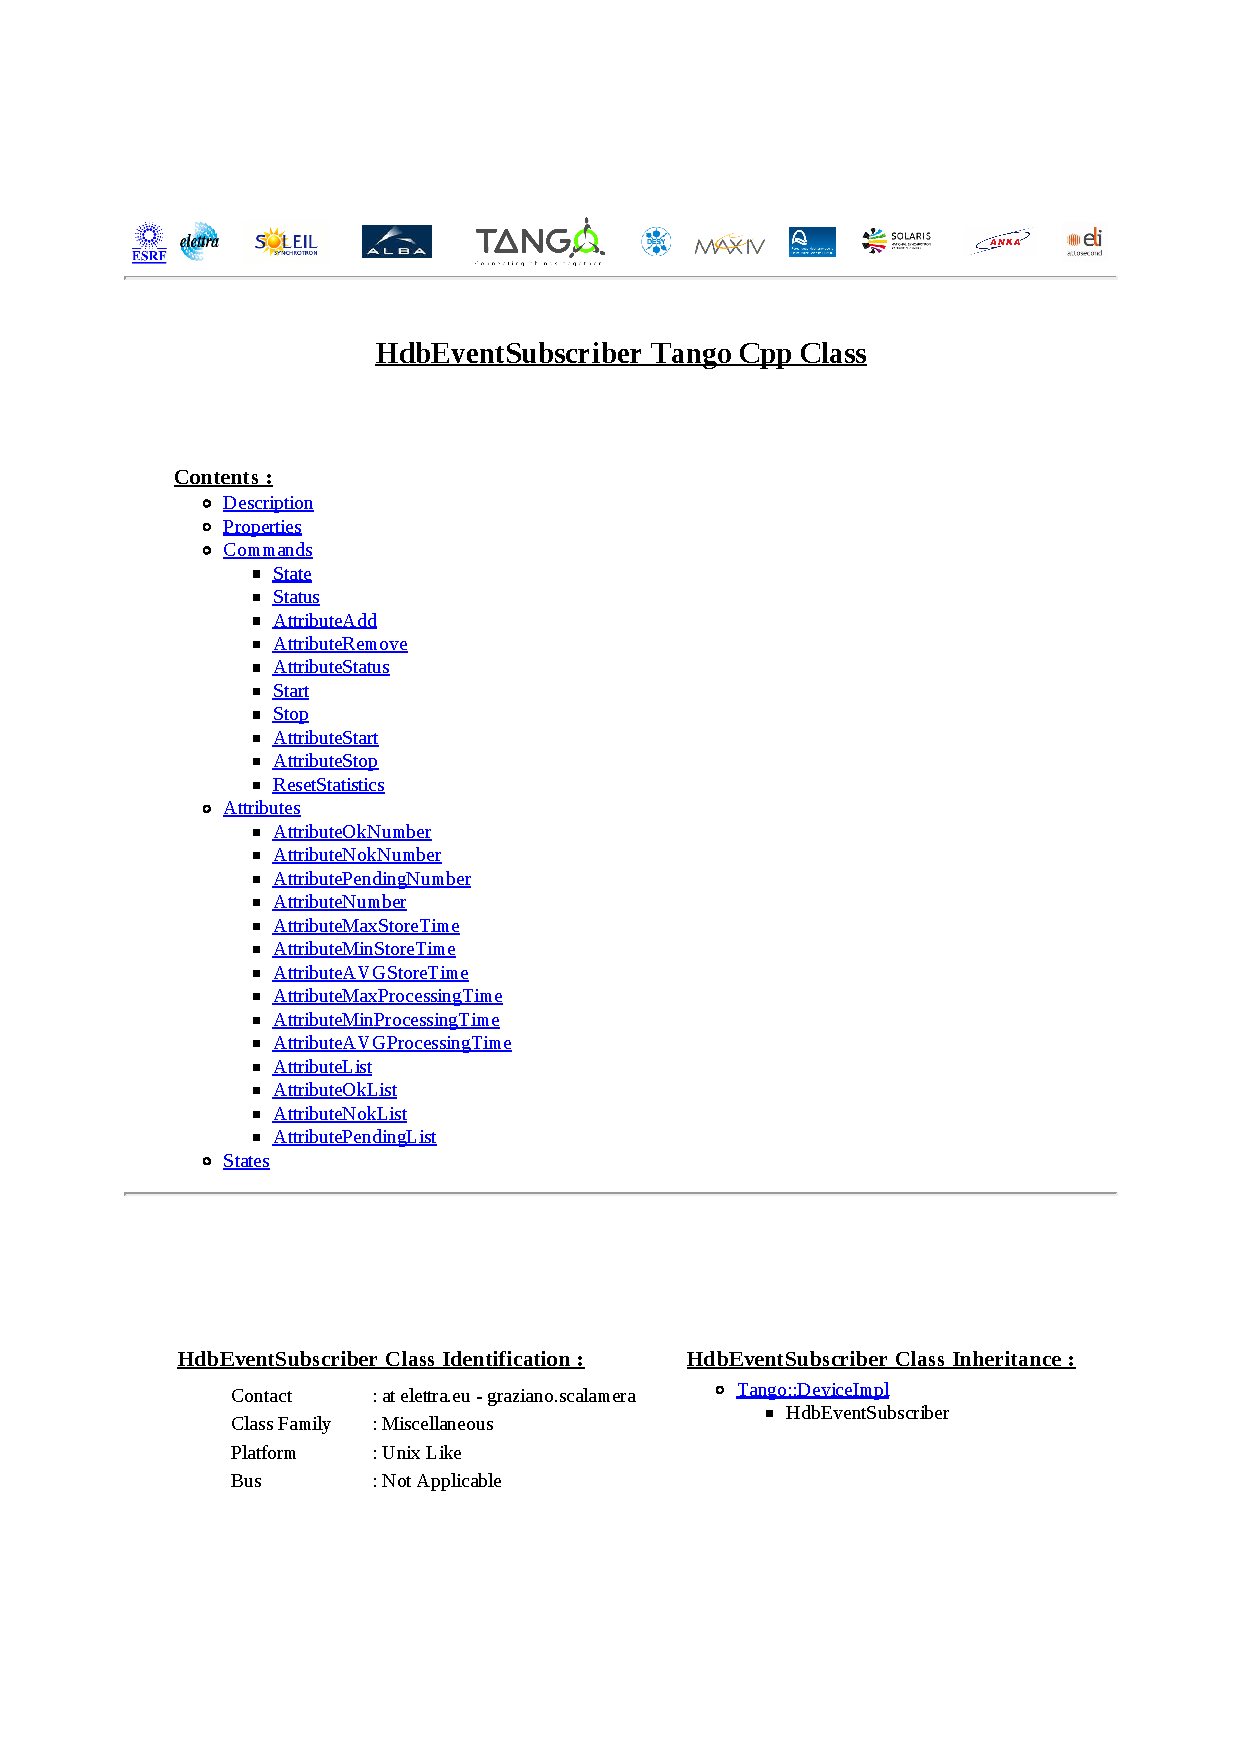
\includepdf[pages={-}]{ES.pdf}

\newpage{\clearpage}

\section{\cm{} full documentation}
\label{app:cmfulldoc}
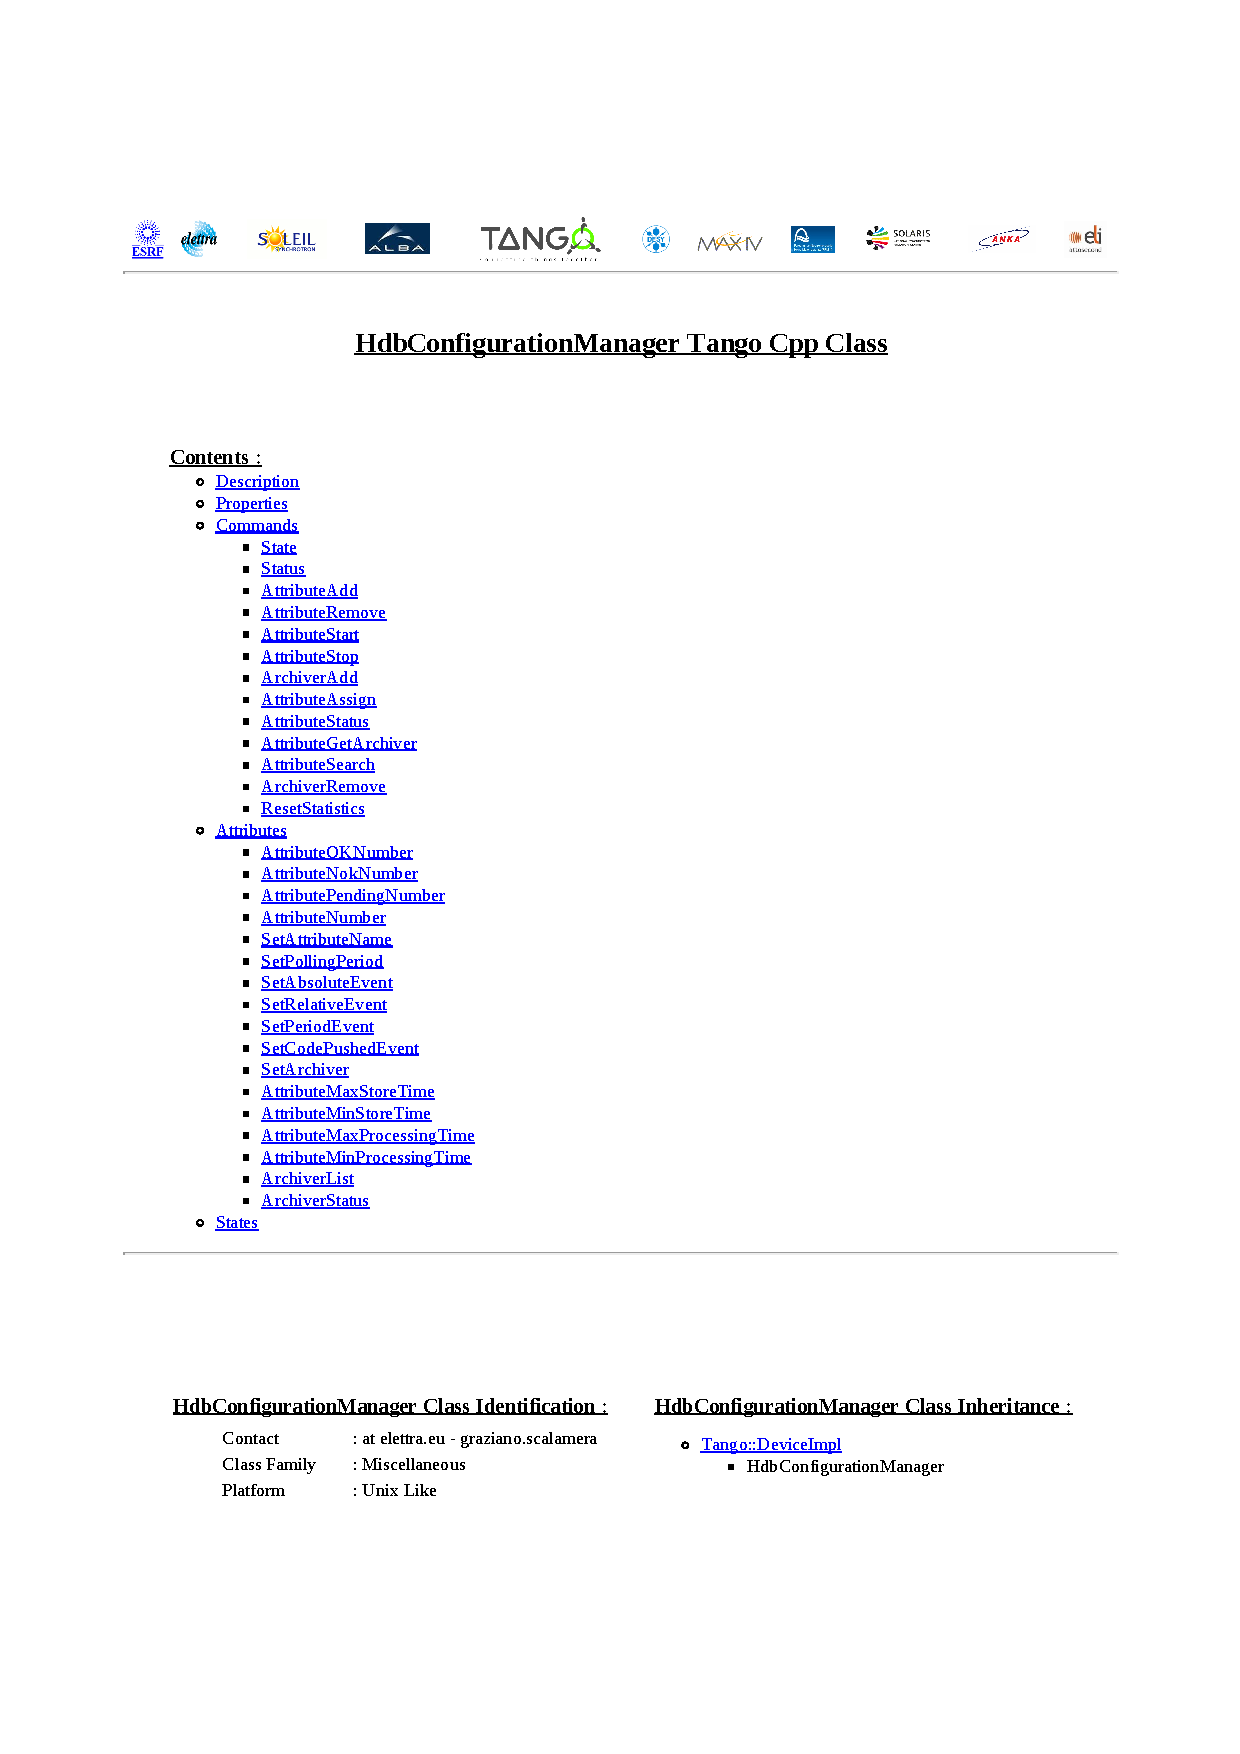
\includepdf[pages={-}]{CM.pdf}

\end{document}








